\documentclass{beamer}
\mode<presentation>
\usepackage{amsmath,amssymb,mathtools}
\usepackage{textcomp}
\usepackage{gensymb}
\usepackage{adjustbox}
\usepackage{subcaption}
\usepackage{enumitem}
\usepackage{multicol}
\usepackage{listings}
\usepackage{url}
\usepackage{graphicx} % <-- needed for images
\def\UrlBreaks{\do\/\do-}

\usetheme{Boadilla}
\usecolortheme{lily}
\setbeamertemplate{footline}{
  \leavevmode%
  \hbox{%
  \begin{beamercolorbox}[wd=\paperwidth,ht=2ex,dp=1ex,right]{author in head/foot}%
    \insertframenumber{} / \inserttotalframenumber\hspace*{2ex}
  \end{beamercolorbox}}%
  \vskip0pt%
}
\setbeamertemplate{navigation symbols}{}

\lstset{
  frame=single,
  breaklines=true,
  columns=fullflexible,
  basicstyle=\ttfamily\tiny   % tiny font so code fits
}

\numberwithin{equation}{section}

% ---- your macros ----
\providecommand{\nCr}[2]{\,^{#1}C_{#2}}
\providecommand{\nPr}[2]{\,^{#1}P_{#2}}
\providecommand{\mbf}{\mathbf}
\providecommand{\pr}[1]{\ensuremath{\Pr\left(#1\right)}}
\providecommand{\qfunc}[1]{\ensuremath{Q\left(#1\right)}}
\providecommand{\sbrak}[1]{\ensuremath{{}\left[#1\right]}}
\providecommand{\lsbrak}[1]{\ensuremath{{}\left[#1\right.}}
\providecommand{\rsbrak}[1]{\ensuremath{\left.#1\right]}}
\providecommand{\brak}[1]{\ensuremath{\left(#1\right)}}
\providecommand{\lbrak}[1]{\ensuremath{\left(#1\right.}}
\providecommand{\rbrak}[1]{\ensuremath{\left.#1\right)}}
\providecommand{\cbrak}[1]{\ensuremath{\left\{#1\right\}}}
\providecommand{\lcbrak}[1]{\ensuremath{\left\{#1\right.}}
\providecommand{\rcbrak}[1]{\ensuremath{\left.#1\right\}}}
\theoremstyle{remark}
\newtheorem{rem}{Remark}
\newcommand{\sgn}{\mathop{\mathrm{sgn}}}
\providecommand{\abs}[1]{\left\vert#1\right\vert}
\providecommand{\res}[1]{\Res\displaylimits_{#1}}
\providecommand{\norm}[1]{\lVert#1\rVert}
\providecommand{\mtx}[1]{\mathbf{#1}}
\providecommand{\mean}[1]{E\left[ #1 \right]}
\providecommand{\fourier}{\overset{\mathcal{F}}{ \rightleftharpoons}}
\providecommand{\system}{\overset{\mathcal{H}}{ \longleftrightarrow}}
\providecommand{\dec}[2]{\ensuremath{\overset{#1}{\underset{#2}{\gtrless}}}}
\newcommand{\myvec}[1]{\ensuremath{\begin{pmatrix}#1\end{pmatrix}}}
\newcommand{\mydet}[1]{\ensuremath{\begin{vmatrix}#1\end{vmatrix}}}

\newenvironment{amatrix}[1]{%
  \left(\begin{array}{@{}*{#1}{c}|*{#1}{c}@{}}
}{%
  \end{array}\right)
}

\newcommand{\myaugvec}[2]{\ensuremath{\begin{amatrix}{#1}#2\end{amatrix}}}
\let\vec\mathbf
% ---------------------

\title{Matgeo Presentation - Problem 9.2.19}
\author{ee25btech11056 - Suraj.N}

\begin{document}

\begin{frame}
  \titlepage
\end{frame}

\begin{frame}{Problem Statement}

Find the area of the smaller part of the circle \(x^{2}+y^{2}=a^{2}\) cut off by the line \(x=\frac{a}{\sqrt{2}}.\)

\end{frame}

\begin{frame}{Data}

\begin{table}[h!]
  \centering
  \begin{tabular}{|c|c|}
\hline
\textbf{Name} & \textbf{Value} \\ \hline
$\vec{A}$ & $\myvec{2 & 1 \\0 & 3}$ \\ \hline
\end{tabular}

  \caption*{Table : Circle}
  \label{9.2.19}
\end{table}

\end{frame}

\begin{frame}{Solution}

The parameters for the circle are :

\begin{align}
  \vec{V} &= \vec{I} & \vec{u} &= \vec{0} & f &= -a^2 
\end{align}

The parameters for the line are :

\begin{align}
  \vec{h} &= \myvec{\tfrac{a}{\sqrt{2}}\\0} & \vec{m} &= \myvec{0\\1}
\end{align}

Substituting these in the below equation to find the intersection points :

\begin{align}
\kappa_i
  &= \frac{1}{\vec{m}^\top \vec{V}\vec{m}}
     \left(
       -\,\vec{m}^\top\big(\vec{V}\vec{h}+\vec{u}\big)
       \;\pm\;
       \sqrt{ \big[\vec{m}^\top(\vec{V}\vec{h}+\vec{u})\big]^2
       - g(\vec{h})\,\big(\vec{m}^\top \vec{V}\vec{m}\big)}
     \right)\\
    g(\vec{x}) &= \vec{x}^\top\vec{x} - a^2 \\
    g(\vec{h}) &= \vec{h}^\top\vec{h} - a^2 
\end{align}

\end{frame}

\begin{frame}{Solution}

\begin{align}
\kappa_i &=\left(
       -\,\vec{m}^\top\vec{h}
       \;\pm\;
       \sqrt{a^2 -\vec{h}^\top\vec{h}}
     \right)\\
  \kappa_i &= \frac{a}{\sqrt{2}},-\frac{a}{\sqrt{2}}
\end{align}

Therefore the points of intersection are :

\begin{align}
  \vec{P_1} &= \myvec{\tfrac{a}{\sqrt{2}}\\\tfrac{a}{\sqrt{2}}} & \vec{P_2} &= \myvec{\tfrac{a}{\sqrt{2}}\\-\tfrac{a}{\sqrt{2}}}
\end{align}

Thus the area of the smaller part of the circle cut off by the line is :

\begin{align}
  2 \int\limits_{\frac{a}{\sqrt{2}}}^{a}\! \sqrt{a^2 - x^2}\, dx &= \frac{a^2}{2}\left(\frac{\pi}{2} - 1\right)
\end{align}

\end{frame}

\begin{frame}{Plot}

\begin{figure}[h!]
  \centering
  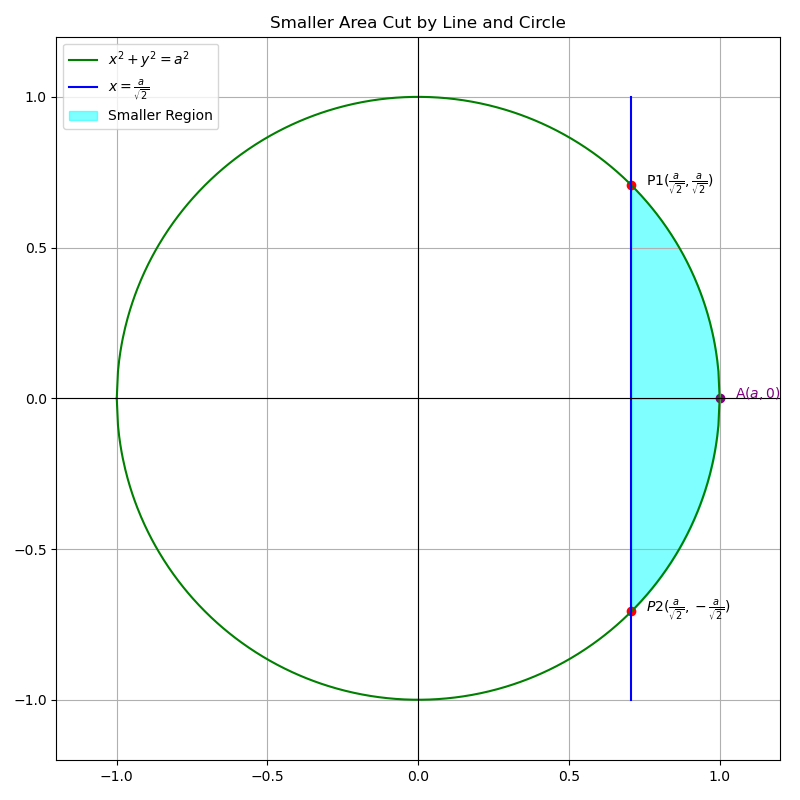
\includegraphics[width=0.6\columnwidth]{figs/circle_area.png} 
   \caption*{Fig : Circle}
  \label{Fig1}
\end{figure}

\end{frame}

\end{document}


